% !TEX root=main.tex

\section{Experimental Results}

Data was collected on a single multirotor agent, shown in~\ref{fig:leo_hardware}.  This agent was flown four times in a cluttered, GPS denied environment.  The agent was initalized in various locations with various initial headings but flew in trajectories which would provide sufficient overlap to calculate loop closures.  The data from each flight was saved and post-processed by the same onboard computer as if all flights were being performed simultaneously by different agents connected to the same ROS network.  The optimized route of each agent can be seen in figure~\ref{fig:hardware_results}.  Each flight took about 2 minutes, and traversed on average about 100m.

\begin{figure}[H]
  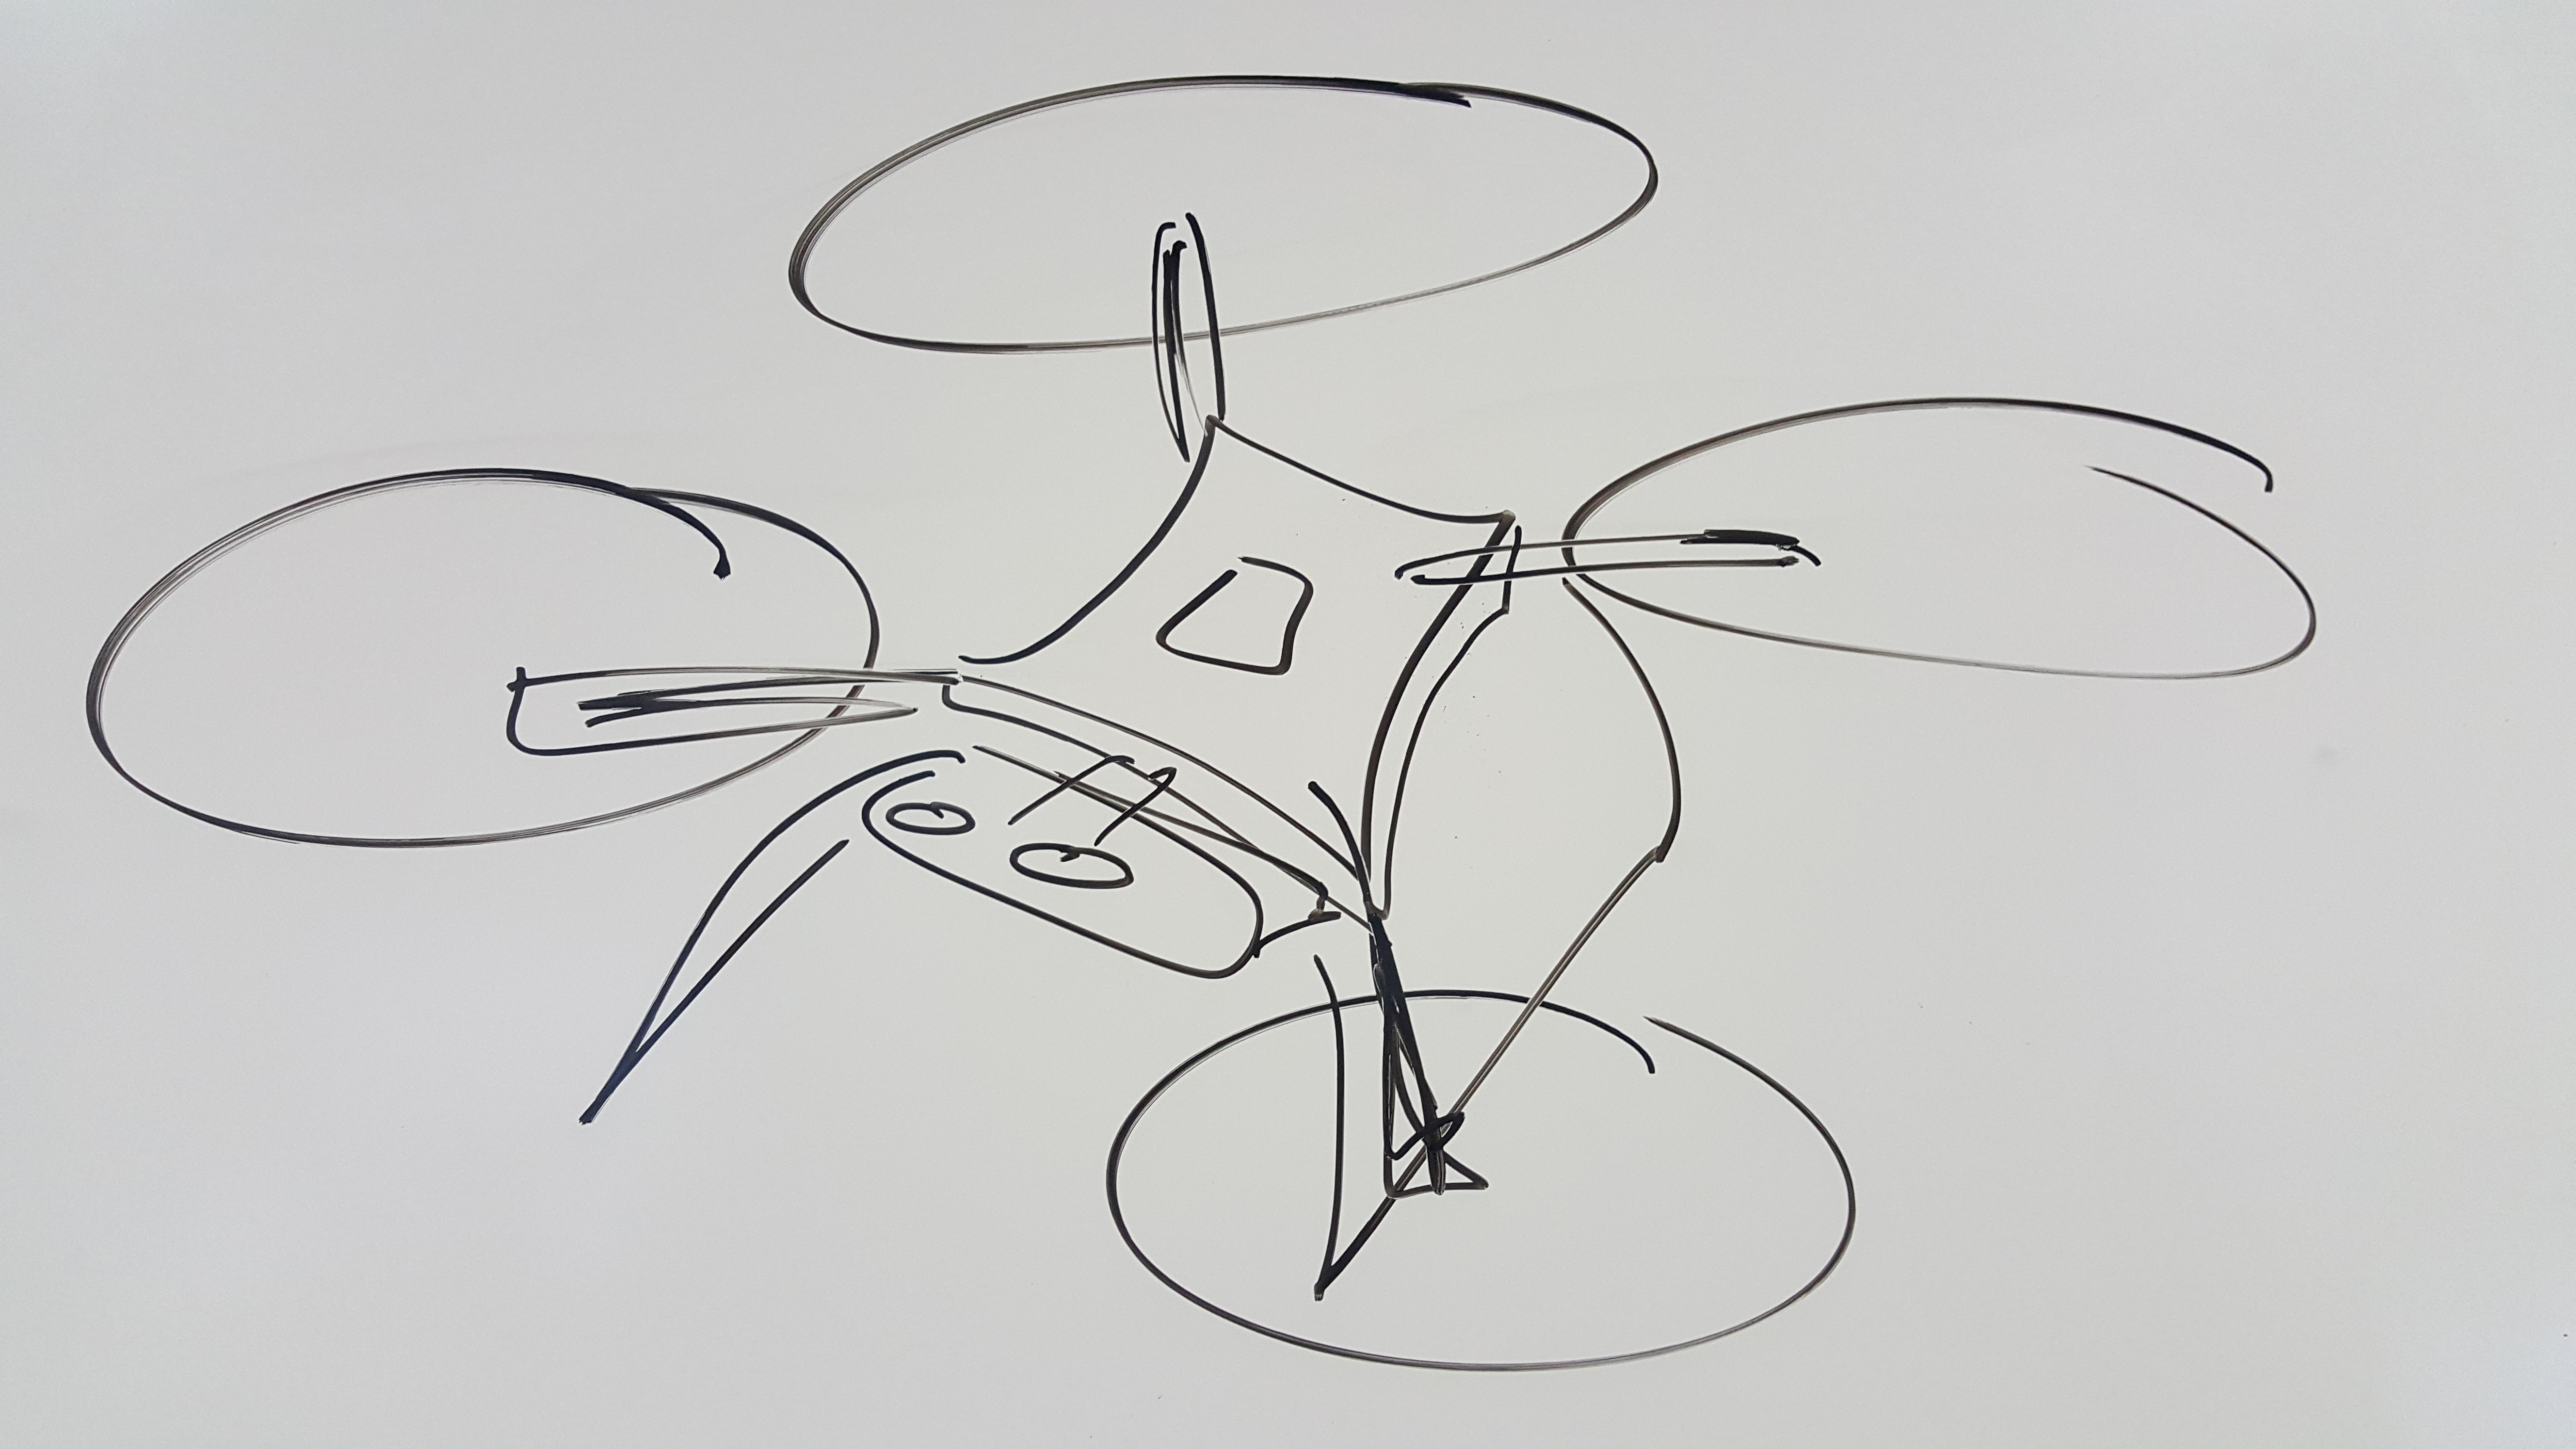
\includegraphics[width=0.7\textwidth]{figures/leo.jpg}
  \caption{Multirotor used in testing.  Processing was performed by an onboard computer with i7-4660U dual core processor and 16GB RAM.  An ASUS XTION RGBD camera was used to provide visual odometry which was fed to an RMEKF which fused MEMS IMU sensor readings and sonar altimeter information collected by a flip32 flight control board running ROSflight.}
  \label{fig:leo_hardware}
\end{figure}


\begin{figure}[H]
  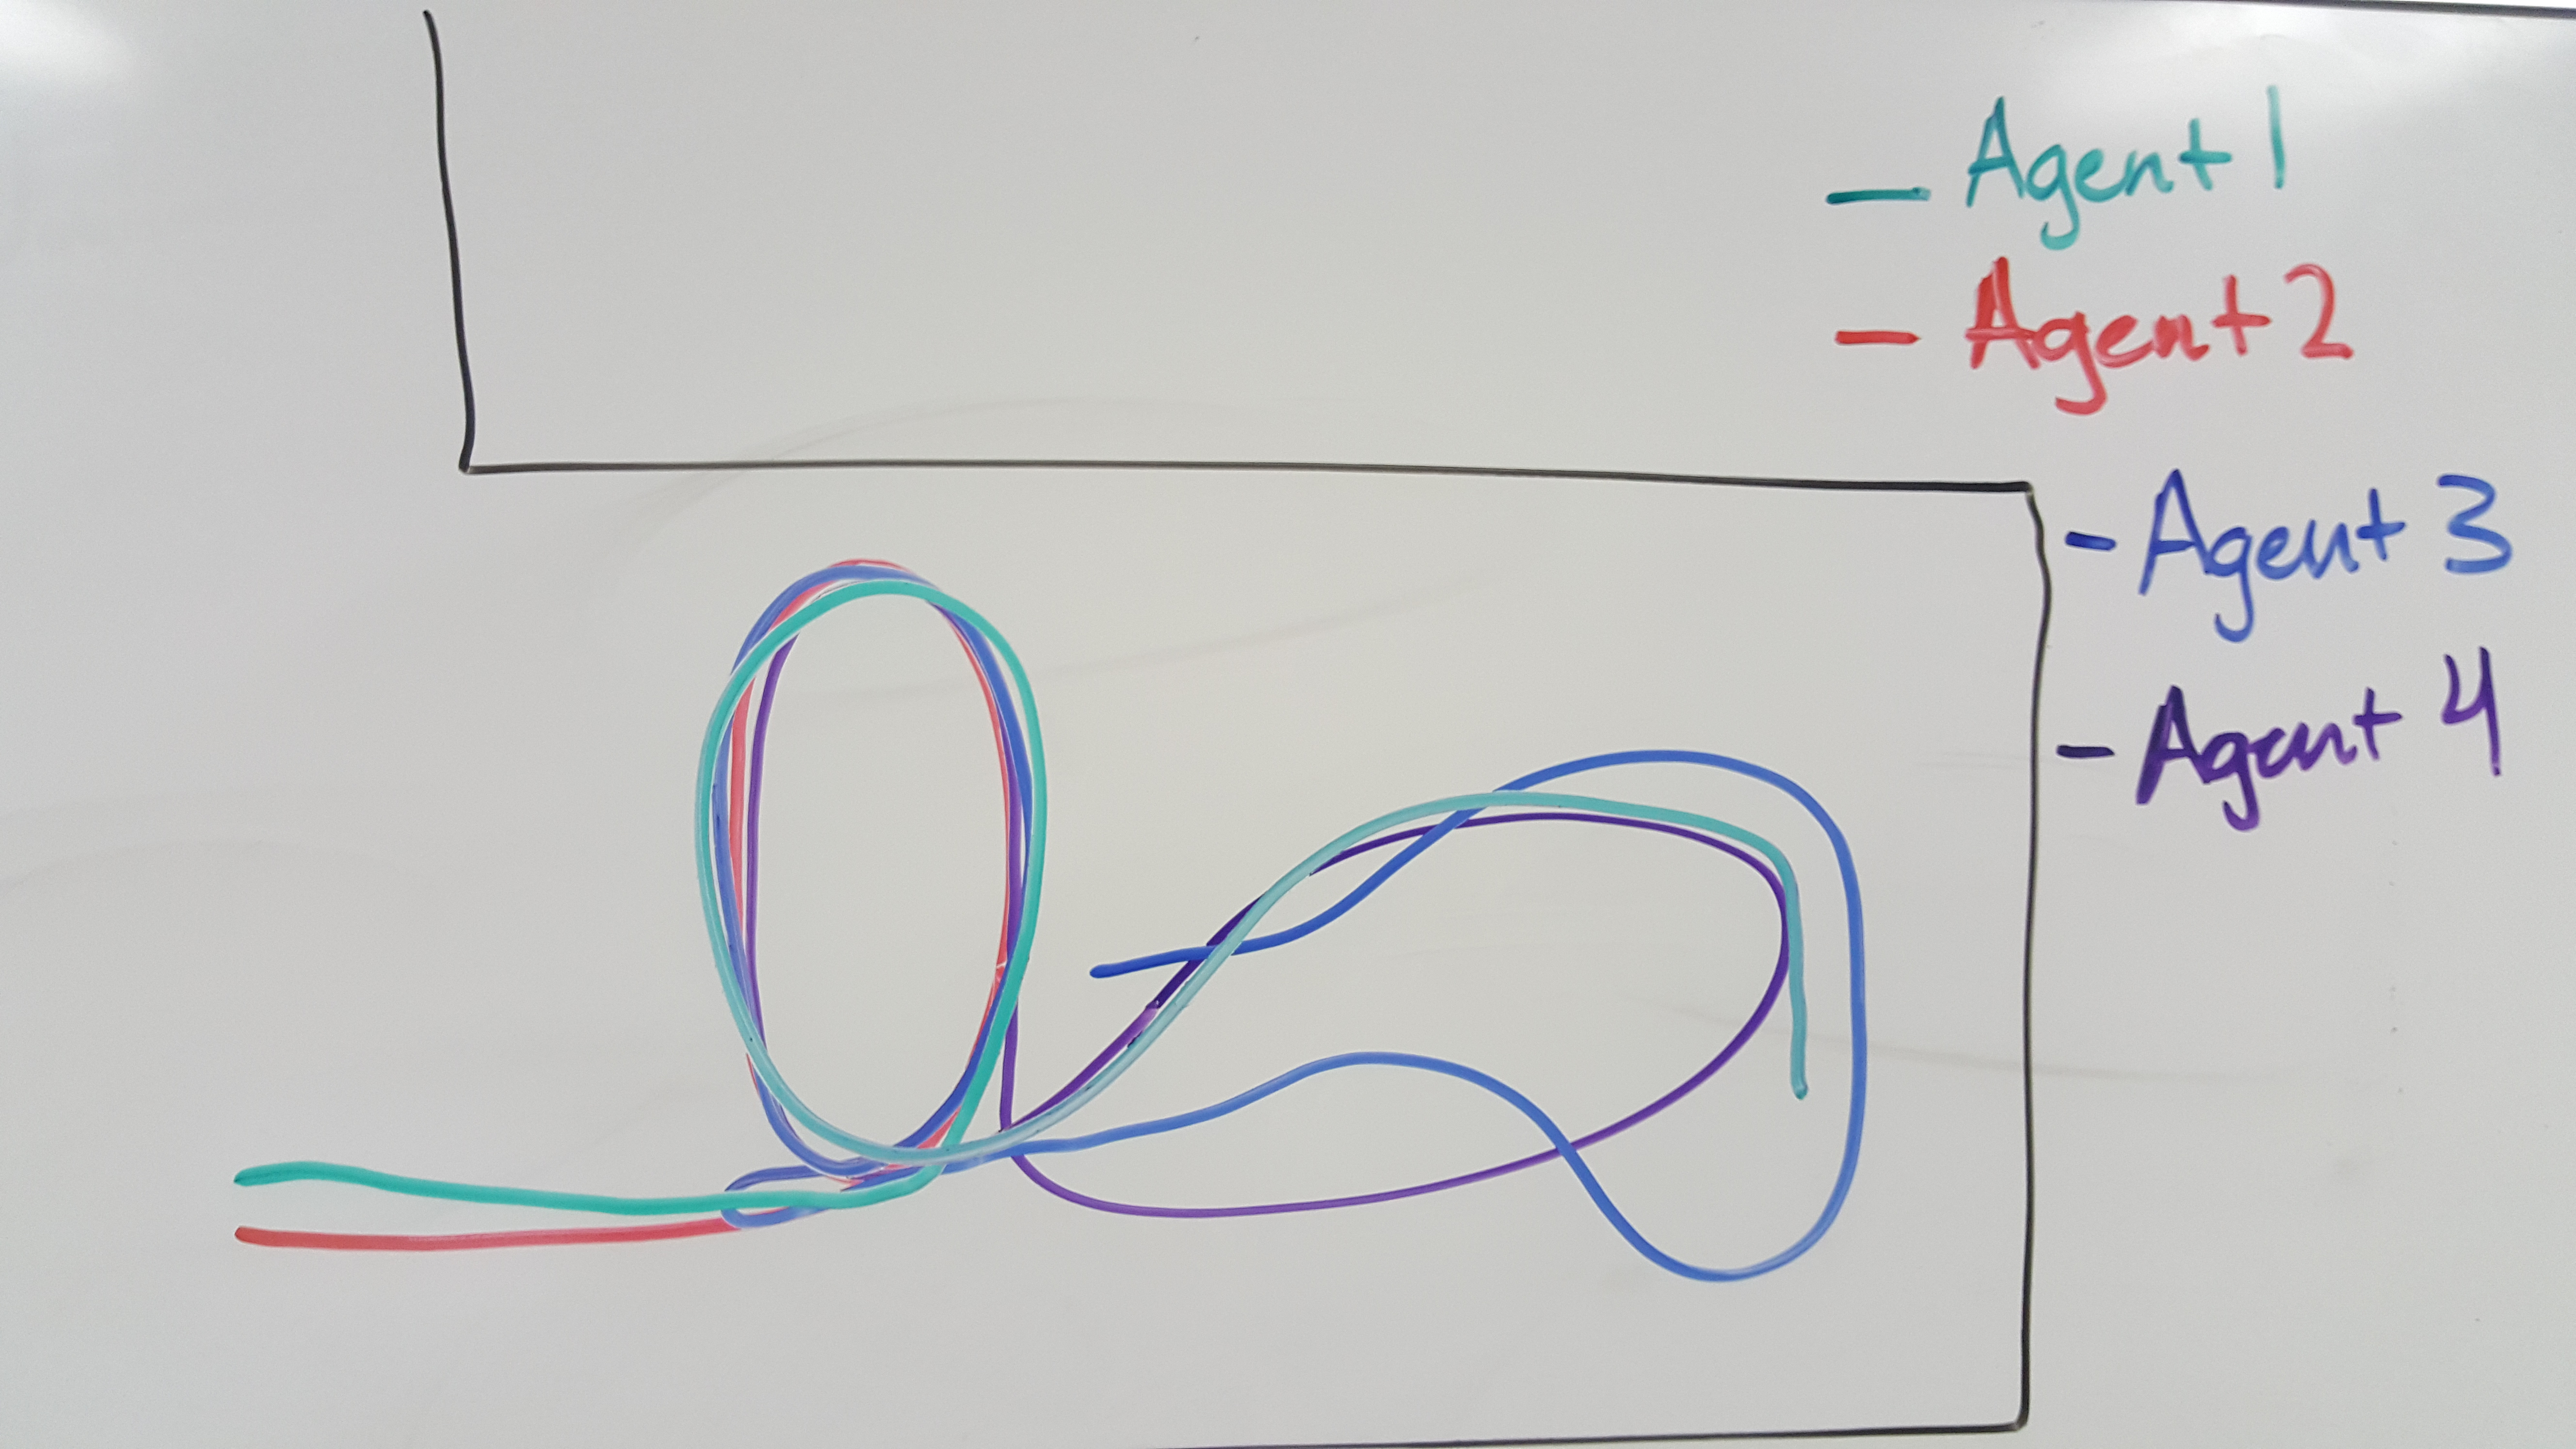
\includegraphics[width=0.7\textwidth]{figures/hardware_results.jpg}
  \caption{Multirotor used in testing.  Processing was performed by an onboard computer with i7-4660U dual core processor and 16GB RAM.  An ASUS XTION RGBD camera was used to provide visual odometry which was fed to an RMEKF which fused MEMS IMU sensor readings and sonar altimeter information collected by a flip32 flight control board running ROSflight.}
  \label{fig:hardware_results}
\end{figure}

This experiment was repeated two times.  In the first experiment, a python implementation of REO was used to as the sole optimization routine.  Optimization was performed once per second on all available information from the perspective of the first agent.  Optimization was performed as a batch, initialized with raw odometry and loop closure measurements.  The optimization always converged in less than 30 iterations for the entirety of the experiment.  On average, optimizations took about 0.1s, but the time to optimization grew as the combined graph got more complicated.

The second experiment used REO only to initialize new agents, aligning them with the primary graph by performing 3 iterations of optimization on the smallest set of edges which forms a loop that includes two agents.   After this initial alignment phase, GPO was used to quickly converge to an estimate.  This resulted in a fixed-cost add to the optimization routine, as the cost of performing REO did not change with increasingly complicated graphs.  GPO also scales non-linearly with increasing graph complexity, but not as strongly as REO.  Therefore it is much more reasonable to use in large networks of agents.

\begin{figure}[H]
  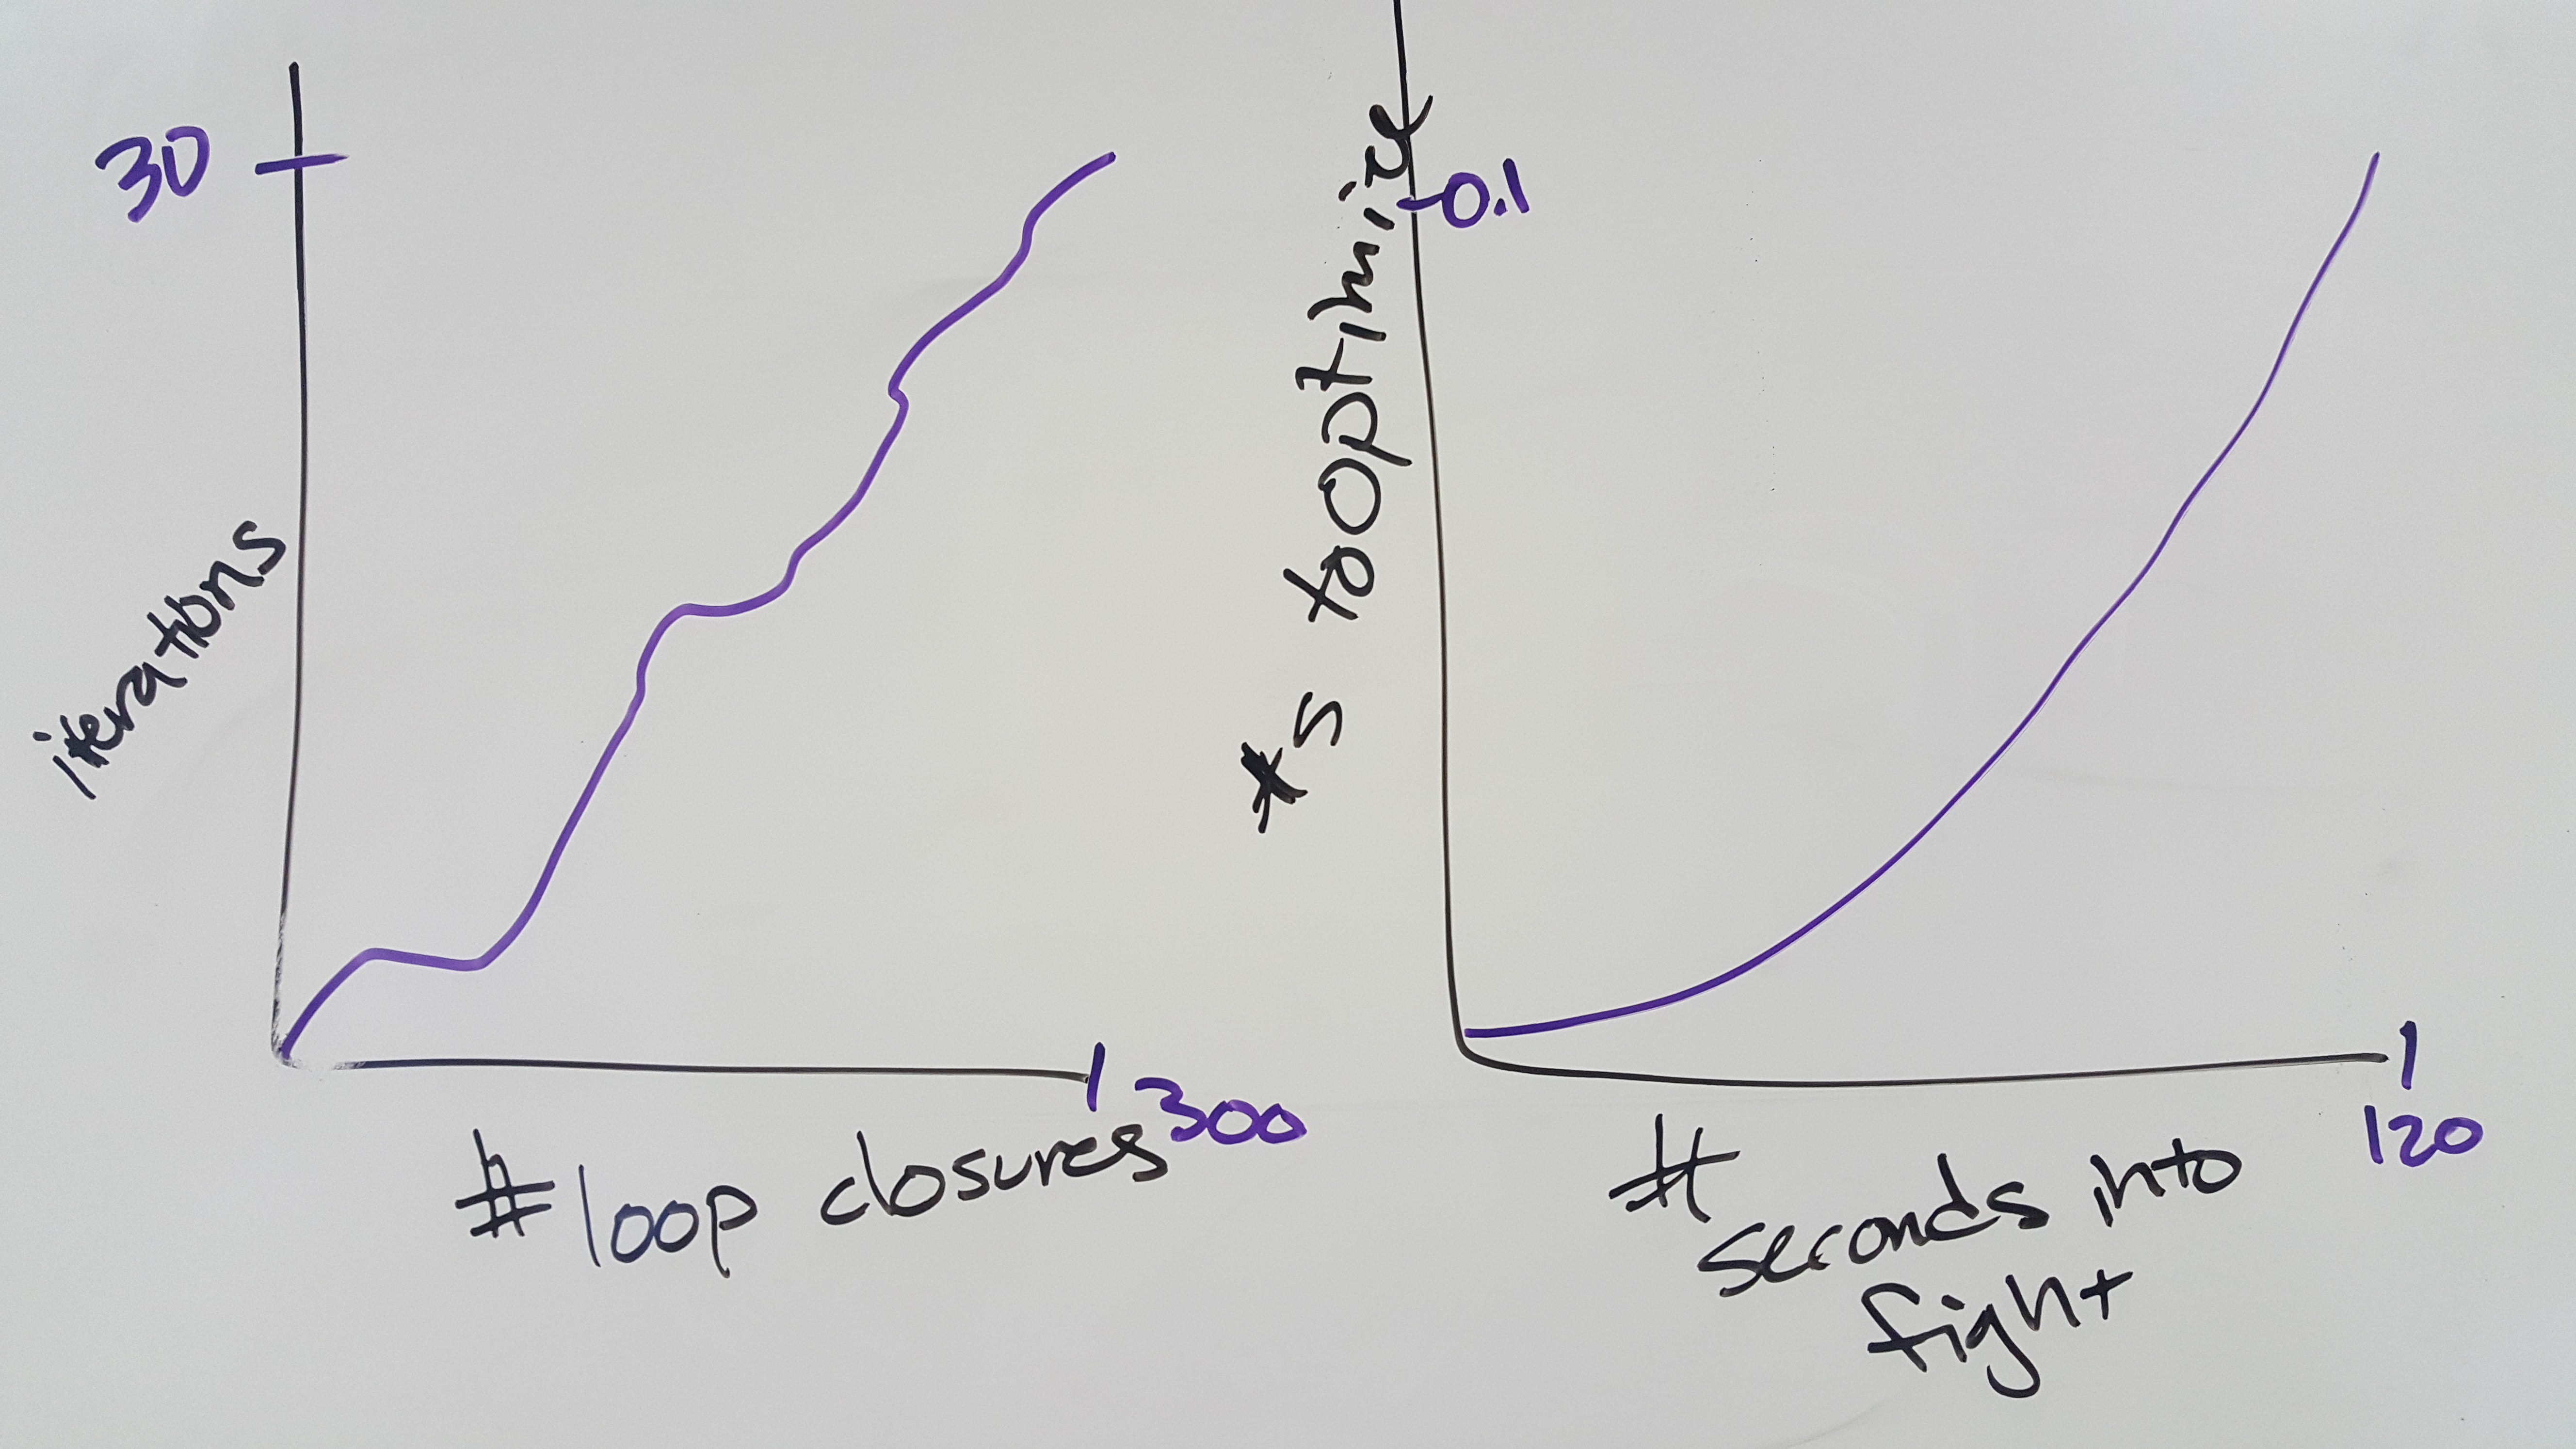
\includegraphics[width=0.7\textwidth]{figures/REO_only_timing_results.jpg}
  \caption{Average number of iterations of REO vs the number of loop closures discovered in the system and average number of seconds to optimize vs the number of seconds into the flight.  While REO was able to perform in real time for this experiment, large scale experiments could pose a challenge for a REO-only backend}
  \label{fig:REO_only_hardware_results}
\end{figure}
